\section{Langkah-Langkah Percobaan}
\section{Langkah-Langkah Percobaan}

\begin{enumerate}
    \item \textbf{Reset Router}

    Pastikan perangkat router telah dikembalikan ke konfigurasi awal untuk mencegah potensi konflik dalam pengaturan selanjutnya.

    \begin{itemize}
        \item Akses router menggunakan aplikasi Winbox.
        \item Navigasikan ke menu \texttt{System > Reset Configuration}.
        \item Aktifkan opsi \texttt{No Default Configuration} dengan mencentangnya.
        \item Klik \texttt{Reset Configuration} untuk memulai proses reset.
    \end{itemize}

    \item \textbf{Login ke Router}

    Lakukan proses login untuk mengakses antarmuka router.

    \begin{itemize}
        \item Gunakan Winbox untuk melakukan koneksi ke router.
        \item Login dapat dilakukan melalui MAC address atau IP default perangkat.
        \item Gunakan username \texttt{admin} (kata sandi tidak diperlukan jika belum diatur).
    \end{itemize}

    \item \textbf{Konfigurasi DHCP Client pada Router A (Ether1)}

    Sambungkan kabel internet ke \texttt{ether1} pada Router A, kemudian lakukan konfigurasi DHCP Client.

    \begin{itemize}
        \item Akses menu \texttt{IP > DHCP Client}.
        \item Klik ikon \texttt{+} untuk menambah entri baru.
        \item Pilih \texttt{ether1} sebagai interface.
        \item Klik \texttt{Apply} dan pastikan status koneksi menunjukkan \texttt{bound}.
    \end{itemize}

    \item \textbf{Penambahan Alamat IP pada Ether7}

    Tambahkan alamat IP pada \texttt{ether7} untuk konektivitas dengan Switch.

    \begin{itemize}
        \item Navigasikan ke menu \texttt{IP > Addresses}.
        \item Klik ikon \texttt{+} untuk menambahkan alamat IP.
        \item Masukkan Address: \texttt{192.168.10.1/24}.
        \item Pilih Interface: \texttt{ether7}.
        \item Klik \texttt{Apply} kemudian \texttt{OK}.
    \end{itemize}

    \item \textbf{Konfigurasi DHCP Server pada Router MikroTik}

    Konfigurasi DHCP Server digunakan untuk secara otomatis mendistribusikan alamat IP kepada perangkat klien.

    \begin{itemize}
        \item Akses menu \texttt{IP > DHCP Server}.
        \item Klik tombol \texttt{DHCP Setup}.
        \item Pilih interface \texttt{ether7}, klik \texttt{Next}.
        \item Verifikasi network address: \texttt{192.168.10.0/24}, klik \texttt{Next}.
        \item Verifikasi gateway: \texttt{192.168.10.1}, klik \texttt{Next}.
        \item Tentukan rentang IP: \texttt{192.168.10.2-192.168.10.254}, klik \texttt{Next}.
        \item Masukkan DNS Server: \texttt{8.8.8.8} dan \texttt{8.8.4.4}, klik \texttt{Next}.
        \item Atur lease time: \texttt{00:10:00}, klik \texttt{Next}.
        \item Setelah selesai, klik \texttt{OK}.
    \end{itemize}

    \item \textbf{Konfigurasi NAT}

    Lakukan konfigurasi NAT (Network Address Translation) untuk menyediakan konektivitas internet.

    \begin{itemize}
        \item Akses menu \texttt{IP > Firewall > NAT}.
        \item Klik ikon \texttt{+} untuk membuat aturan baru.
        \item Pada tab \texttt{General}, atur Chain: \texttt{src-nat}.
        \item Pada tab \texttt{Action}, atur Action: \texttt{masquerade}.
        \item Klik \texttt{Apply} kemudian \texttt{OK}.
        \item Untuk uji koneksi, buka terminal di Winbox dan gunakan perintah \texttt{ping 8.8.8.8}.
    \end{itemize}

    \item \textbf{Konfigurasi Firewall}

    Tambahkan aturan filter (Filter Rules) pada firewall.

    \begin{itemize}
        \item \textbf{Pemblokiran ICMP:}
        \begin{itemize}
            \item Akses menu \texttt{IP > Firewall > Filter Rule}.
            \item Klik ikon \texttt{+} untuk menambahkan aturan baru.
            \item Pada tab \texttt{General}, atur Chain: \texttt{forward}, Protocol: \texttt{icmp}, dan In. Interface: \texttt{ether7}.
            \item Pada tab \texttt{Action}, atur Action: \texttt{drop}.
        \end{itemize}
        \item \textbf{Pemblokiran Konten Web (Content Blocking):}
        \begin{itemize}
            \item Tambahkan aturan baru pada tab \texttt{Filter Rule}.
            \item Pada tab \texttt{General}, atur Chain: \texttt{forward}, Protocol: \texttt{tcp}, Dst. Port: \texttt{80,443}, In. Interface: \texttt{ether7}, dan Out. Interface: \texttt{ether1}.
            \item Pada tab \texttt{Advanced}, atur Content: \texttt{speedtest}.
            \item Pada tab \texttt{Action}, atur Action: \texttt{drop}.
        \end{itemize}
    \end{itemize}

    \item \textbf{Konfigurasi Bridge pada Router B}

    Lakukan konfigurasi bridge untuk menjadikan Router B sebagai hub.

    \begin{itemize}
        \item Akses menu \texttt{Bridge}.
        \item Klik ikon \texttt{+} untuk membuat bridge baru, lalu klik \texttt{Apply} dan \texttt{OK}.
        \item Akses menu \texttt{Bridge > Port}.
        \item Tambahkan interface yang terhubung ke perangkat laptop dan interface yang terhubung ke Router A.
    \end{itemize}

    \item \textbf{Konfigurasi Alamat IP pada Laptop}

    \begin{itemize}
        \item Atur pengaturan jaringan pada laptop agar menggunakan DHCP (otomatis).
        \item Buka Command Prompt (CMD).
        \item Gunakan perintah \texttt{ipconfig} untuk memverifikasi alamat IP yang diperoleh.
    \end{itemize}

    \item \textbf{Uji Coba Konfigurasi}

    \begin{itemize}
        \item \textbf{Pengujian Konektivitas (ICMP):}
        \begin{itemize}
            \item Buka terminal pada laptop.
            \item Jalankan perintah \texttt{ping 8.8.8.8}.
            \item Jika firewall ICMP aktif, hasil yang diharapkan adalah \texttt{Request Timed Out}.
            \item Nonaktifkan aturan firewall ICMP dengan menekan tanda "X" (disable).
            \item Ulangi ping untuk memastikan koneksi berhasil.
        \end{itemize}
        \item \textbf{Pengujian Pemblokiran Konten Web:}
        \begin{itemize}
            \item Akses situs web dengan kata kunci \texttt{speedtest} (misalnya: \texttt{www.speedtest.net}).
            \item Jika firewall konten aktif, akses akan gagal atau tidak memuat sempurna.
            \item Nonaktifkan aturan firewall konten untuk menguji akses normal kembali.
        \end{itemize}
    \end{itemize}
\end{enumerate}

\section{Analisis Hasil Percobaan}

Dari hasil percobaan yang dilakukan, dapat disimpulkan bahwa seluruh tahapan konfigurasi router MikroTik berjalan dengan baik dan sesuai ekspektasi. Proses reset router memastikan perangkat dalam kondisi bersih tanpa konfigurasi sebelumnya, sehingga meminimalkan potensi konflik konfigurasi. Proses login melalui Winbox juga tidak mengalami kendala, memungkinkan praktikan langsung mengakses pengaturan router.

Konfigurasi DHCP Client pada \texttt{ether1} berhasil dilakukan dan router memperoleh IP publik dari jaringan luar, yang menjadi dasar agar perangkat di jaringan lokal dapat terkoneksi ke internet. Selanjutnya, konfigurasi alamat IP statis pada \texttt{ether7} serta pengaktifan DHCP Server menunjukkan bahwa router mampu membagikan IP secara otomatis ke klien melalui jaringan lokal, dibuktikan dengan klien berhasil mendapatkan IP dari rentang yang telah ditentukan.

Penerapan NAT menggunakan metode \texttt{masquerade} juga terbukti efektif, di mana klien dapat mengakses internet menggunakan IP publik yang dimiliki router. Hal ini dibuktikan melalui uji coba perintah \texttt{ping 8.8.8.8} yang berhasil mendapatkan balasan. Pengujian firewall menunjukkan bahwa aturan pemblokiran dapat bekerja sesuai dengan konfigurasi. Ketika aturan pemblokiran ICMP diaktifkan, klien tidak dapat melakukan ping, dan saat aturan dinonaktifkan, koneksi kembali berjalan normal. Begitu juga dengan pemblokiran akses terhadap konten tertentu seperti “speedtest” yang berhasil membatasi akses sesuai filter yang diterapkan.

Secara keseluruhan, percobaan ini menunjukkan bahwa MikroTik dapat dikonfigurasi untuk mengatur distribusi IP, koneksi internet melalui NAT, serta pembatasan akses melalui firewall. Hal ini membuktikan bahwa router MikroTik adalah perangkat yang fleksibel dan dapat diandalkan dalam manajemen jaringan skala kecil hingga menengah. Praktikum ini memberikan pemahaman langsung mengenai konsep dasar jaringan dan implementasinya secara praktis.

\section{Hasil Tugas Modul}
\subsection{Topologi Jaringan}
\begin{figure}[H]
\centering
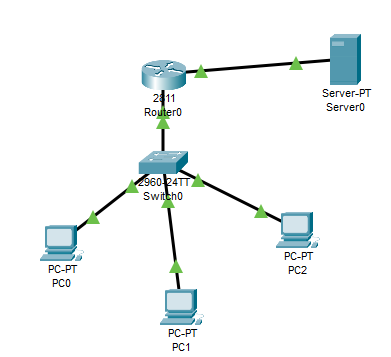
\includegraphics[width=0.8\textwidth]{P1/img/3.png}
\end{figure}

\subsection{Konfigurasi NAT}
\begin{lstlisting}
# Langkah 1: Tentukan interface 'inside' (dari LAN) dan 'outside' (ke Public)
interface FastEthernet0/0
 ip nat inside
exit

interface FastEthernet0/1
 ip nat outside
exit

# Langkah 2: Buat Access Control List (ACL) untuk mengidentifikasi trafik dari LAN yang boleh di-NAT
# ACL Standar nomor 1 ini mengizinkan semua IP dari jaringan 192.168.10.0
access-list 1 permit 192.168.10.0 0.0.0.255

# Langkah 3: Terapkan aturan NAT
# Perintah ini menerjemahkan IP sumber (source) yang cocok dengan ACL 1
# ke alamat IP pada interface FastEthernet0/1 secara overload (PAT)
ip nat inside source list 1 interface FastEthernet0/1 overload
\end{lstlisting}
\begin{figure}[H]
\centering
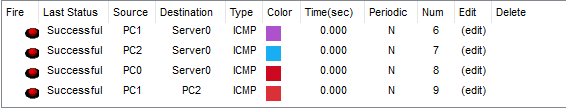
\includegraphics[width=0.8\textwidth]{P1/img/2.png}
\end{figure}
\subsection{Konfigurasi Firewall Access Control List (ACL)}
\begin{lstlisting}
# Buat ACL Extended dengan nama 'FIREWALL_SERVER'
ip access-list extended FIREWALL_SERVER

# Aturan 1: Izinkan PC1 (192.168.10.11) mengakses protokol apa pun (ip) ke Server (200.100.50.2)
permit ip host 192.168.10.11 host 200.100.50.2

# Aturan 2: Tolak/Blokir PC0 (192.168.10.10) mengakses Server
deny ip host 192.168.10.10 host 200.100.50.2

# Aturan 3: Tolak/Blokir PC2 (192.168.10.12) mengakses Server
deny ip host 192.168.10.12 host 200.100.50.2

# Aturan 4: Izinkan semua trafik lain yang berasal dari LAN
# Ini penting agar proses NAT untuk PC1 tetap berjalan dan tidak terblokir
permit ip 192.168.10.0 0.0.0.255 any

# Terapkan ACL ini pada interface yang mengarah ke Server (Public)
# Arahnya 'in' karena kita menyaring paket yang MASUK ke interface ini dari sisi LAN
interface FastEthernet0/0
 ip access-group FIREWALL_SERVER in
exit
\end{lstlisting}
\begin{figure}[H]
\centering
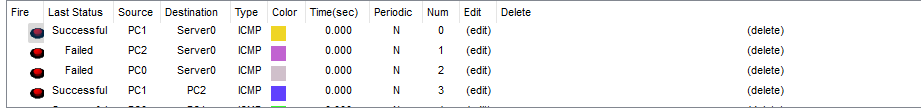
\includegraphics[width=0.8\textwidth]{P1/img/1.png}
\end{figure}
\section{Kesimpulan}

Berdasarkan hasil percobaan yang telah dilakukan, dapat disimpulkan bahwa router MikroTik mampu dikonfigurasi secara efektif untuk memenuhi kebutuhan jaringan lokal, mulai dari distribusi alamat IP secara otomatis menggunakan DHCP Server, konektivitas internet melalui konfigurasi NAT, hingga pengaturan keamanan akses menggunakan firewall. Semua fitur utama berjalan dengan baik dan dapat diuji langsung oleh perangkat klien, baik dari sisi konektivitas maupun pembatasan akses.

Konfigurasi NAT memungkinkan perangkat di jaringan lokal untuk menggunakan satu IP publik dalam mengakses internet, sedangkan fitur firewall memberikan kontrol penuh terhadap lalu lintas data yang masuk maupun keluar. Dengan demikian, percobaan ini memberikan gambaran nyata tentang bagaimana perangkat MikroTik dap
\section{Lampiran}
\subsection{Dokumentasi saat praktikum}
% \begin{figure}[H]
% \centering
% 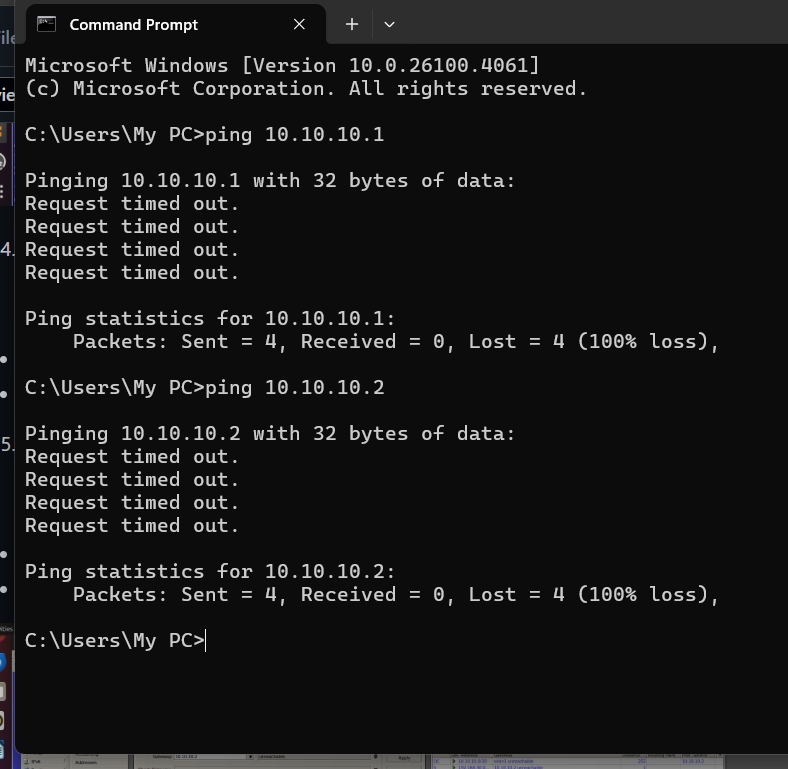
\includegraphics[width=0.8\textwidth]{P1/img/4.png}

% \end{figure}
\begin{figure}[H]
\centering
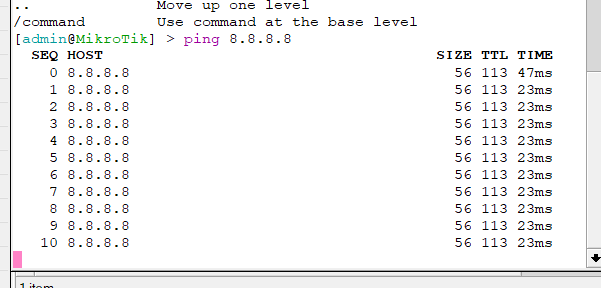
\includegraphics[width=0.8\textwidth]{P1/img/5.png}

\end{figure}
\begin{figure}[H]
\centering
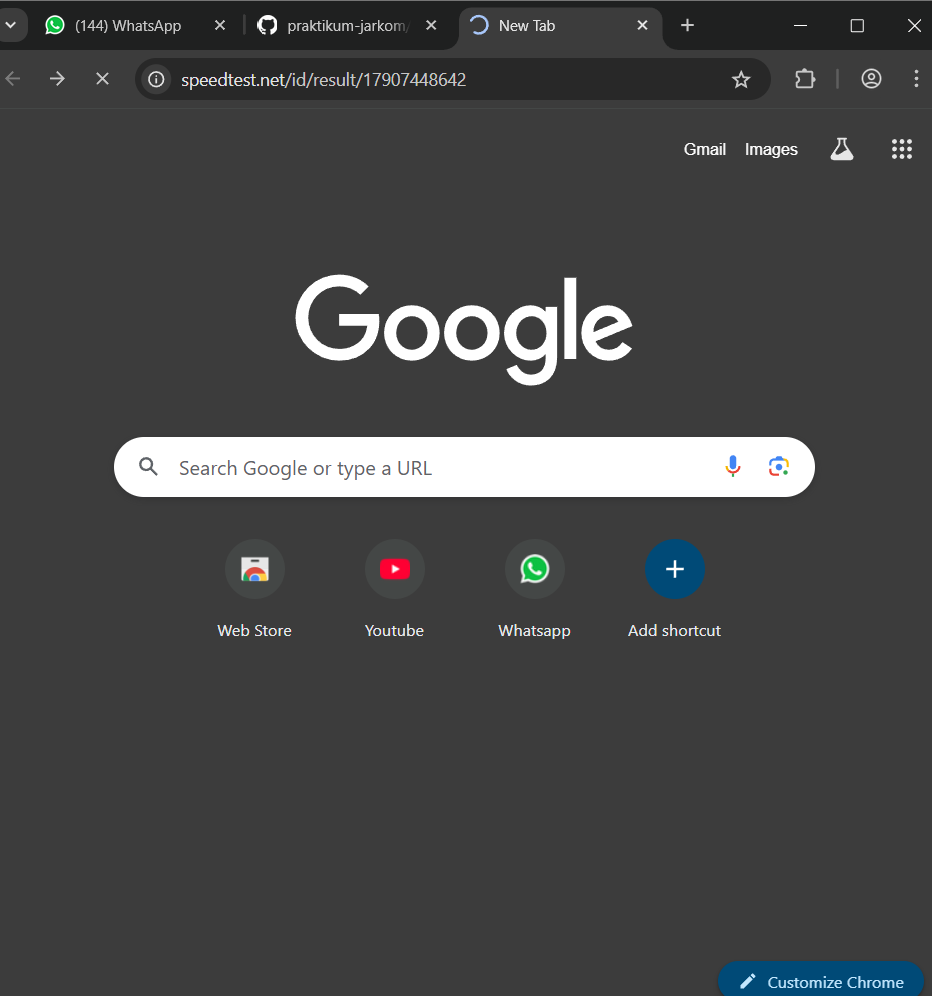
\includegraphics[width=0.8\textwidth]{P1/img/6.png}

\end{figure}
% \begin{figure}[H]
% \centering
% 
\includegraphics[width=0.8\textwidth]{P1/img/7.png}

% \end{figure}
\begin{figure}[H]
\centering
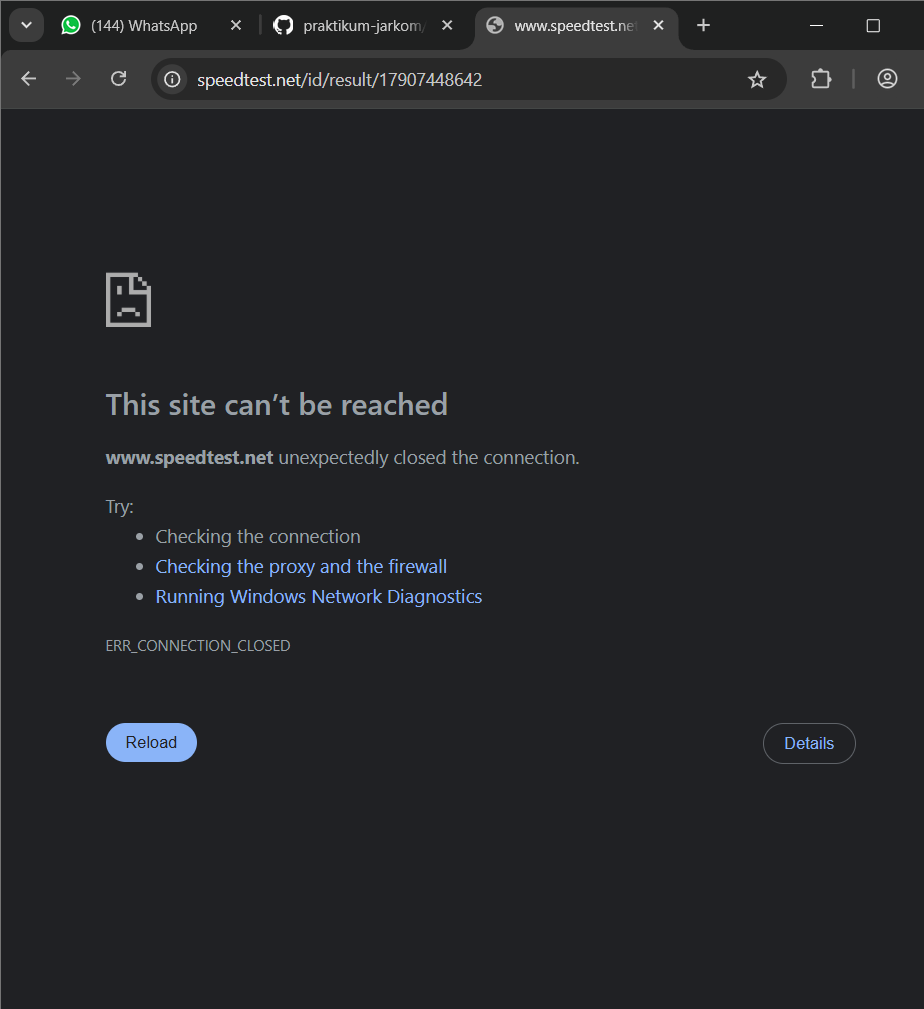
\includegraphics[width=0.8\textwidth]{P1/img/8.png}
 
\end{figure}
\begin{figure}[H]
\centering
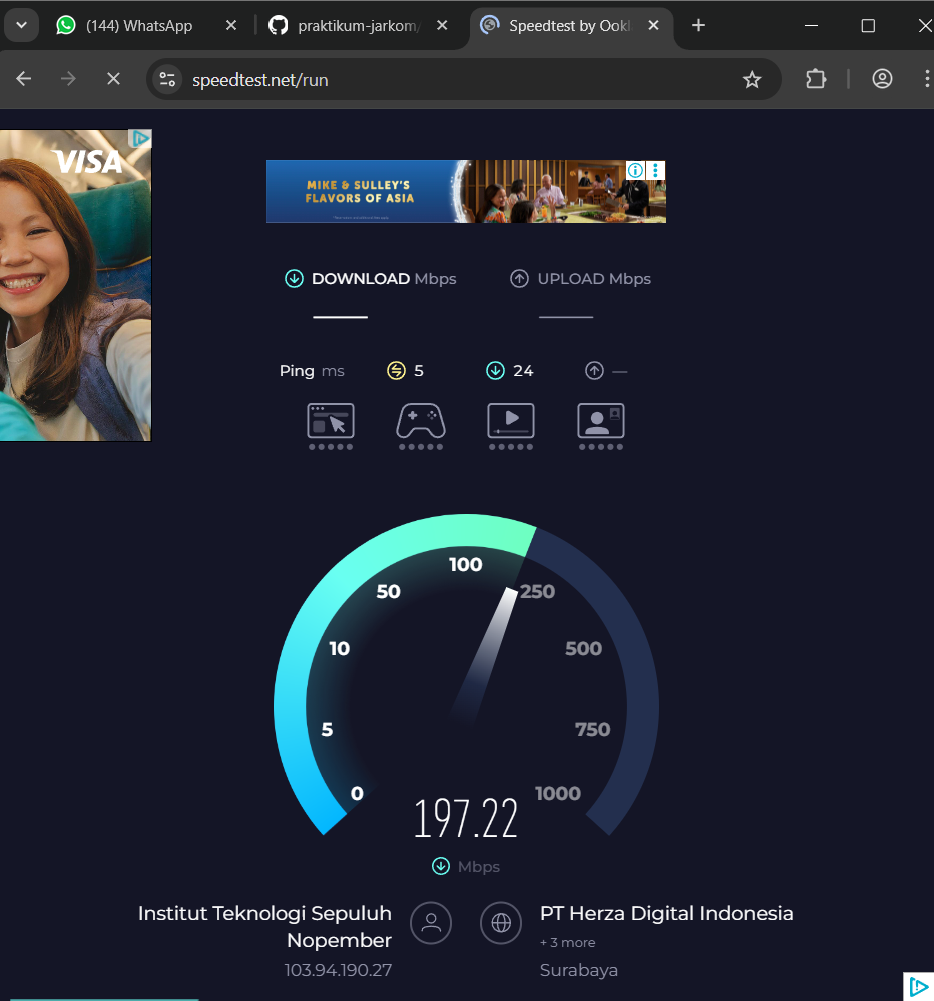
\includegraphics[width=0.8\textwidth]{P1/img/9.png}

\end{figure}